%%%%%%%%%%%%%%%%%%%%%%%%%%%%%%%%%%%%%%%%%%%%%%%%%%%
%%% EVALUACION
%%%%%%%%%%%%%%%%%%%%%%%%%%%%%%%%%%%%%%%%%%%%%%%%%%%

\chapter{Evaluación}
\fancyhead[RE]{\textsc{CAPÍTULO} \thechapter. Evaluación}
\label{ch:Evaluacion}

\noindent Este capítulo describe la metodología utilizada para evaluar el sistema/método o caso de estudio propuesto, a la vez que presenta los resultados obtenidos en la evaluación de las diferentes tareas y sobre colecciones de evaluación de distintos dominios. Algunos ejemplos de secciones pueden ser estos:

% \section{Metodología de evaluación}
% \label{sec:Met_Eval}

% \section{Métricas de evaluación}
% \label{sec:Metric_Eval}

% \section{Colecciones de evaluación}
% \label{sec:Col_Eval}

% \section{Resultados}
% \label{sec:Resultados}

Se han evaluado todos los modelos conseguidos sobre el conjunto de validacion y se pueden ver en al tabla evaluation\_results.csv en la carpeta models-results.

Se han entrenado todos los modelos una unica epoca para evitar el sobreajuste. En la carpeta de imagenes hay algunos ejemplos de overfiting con la funcion de perdida. Los resultados de los modelos entrenados se pueden ver en la tabla finetuned\_results.csv en la carpeta models-results.

Se han elegido los tres primeros modelos con mejores resultados para hacer el ranking fusion.

\section{Entorno de desarrollo}

Todas las evaluaciones que aquí se muestran han sido realizadas en un entorno virtual de Google Colab \cite{googlecolab} con las características que se muestran en la tabla \ref{tab:especificaciones_sistema}.

\begin{table}[ht]
    \centering
    \begin{tabular}{|l|l|}
        \hline
        \textbf{Componente} & \textbf{Especificación}      \\ \hline
        Memoria RAM         & 12 GB                        \\ \hline
        GPU                 & NVIDIA Tesla T4 (15 GB VRAM) \\ \hline
        Sistema operativo   & Ubuntu 22.04.4 LTS           \\ \hline
        Intérprete          & Python 3.12.12               \\ \hline
    \end{tabular}
    \caption{Especificaciones del sistema}
    \label{tab:especificaciones_sistema}
\end{table}

Debido a las limitaciones de memoria y tiempo de ejecución impuestas por Google Colab, se han realizado ciertas adaptaciones en los modelos y conjuntos de datos para asegurar que las evaluaciones pudieran llevarse a cabo de manera eficiente dentro de este entorno. Estas adaptaciones incluyen la no evaluación de modelos con un tamaño excesivo que superaran la memoria disponible, así como de aquellos con los que no sería viable una inferencia posterior dentro de los límites de tiempo establecidos por la plataforma.

\section{Evaluación Zero-Shot}

\subsection{Obtención de modelos preentrenados}

Para esta primera etapa se han evaluado una serie de modelos preentrenados que no han sido sometidos a ningún tipo de alteración o ajuste mediante datos externos. Estos modelos han sido obtenidos a través de la plataforma Hugging Face \cite{huggingface} mediante el uso de la librería Transformers. Esta lista se ha obtenido principalmente de dos fuentes de datos.

La primera fuente, y que ocupa más de la mitad de la lista, ha sido a través del repositorio del MTEB Leaderboard \cite{mteb-leaderboard}, que recopila una gran variedad de modelos preentrenados para tareas de representación y evaluación de texto, evaluados sobre benchmarks estandarizados, proporcionando un ranking actualizado y confiable. Estos modelos, filtrados por aquellos con licencia de uso pública, han sido ordenados y seleccionados los 100 mejores según su desempeño medio en los siguientes benchmarks\footnote{La tabla de resultados ha sido descargada a día 1 de Diciembre de 2025. Se pueden consultar sus valores medios en las métricas en la tabla \ref{tab:resultados_completos_modelos_mteb_retrieval}.}:

\begin{itemize}
    \item BELEBELE Retrieval
    \item Core17 Instruction Retrieval
    \item Covid Retrieval
    \item HAGRID Retrieval
    \item LEMB Passkey Retrieval
    \item MIRACL Retrieval Hard Negatives
    \item MLQA Retrieval
    \item News21 Instruction Retrieval
    \item Robust04 Instruction Retrieval
    \item Statcan Dialogue Dataset Retrieval
    \item Twitter Hjerne Retrieval
    \item TREC COVID
    \item Wikipedia Retrieval Multilingual
\end{itemize}

Esta lista ha sido complementada con una segunda fuente, que se ha basado en la búsqueda automatizada de modelos preentrenados en Hugging Face, que cumplieran los siguientes criterios:

\begin{itemize}
    \item Modelos basados en arquitecturas de transformers.
    \item Modelos diseñados para la tarea de \textit{Sentence Similarity}.
    \item Modelos que hayan sido entrenados con datos en español.
\end{itemize}

En su conjunto, estas dos fuentes han permitido la creación de una lista diversa y representativa de modelos preentrenados para su evaluación en la tarea, proporcionando una base sólida para el análisis comparativo en las siguientes secciones. 

Una vez limpiados de la lista los modelos que no cumplían los requisitos de memoria y tiempo de ejecución, así como configuraciones erróneas, se ha obtenido un total de 190 modelos preentrenados para su evaluación sobre la métrica \gls{MAP}. Podemos ver los resultados obtenidos en la gráfica \ref{fig:zero_shot_map}.

\begin{figure}[H]
    \centering
    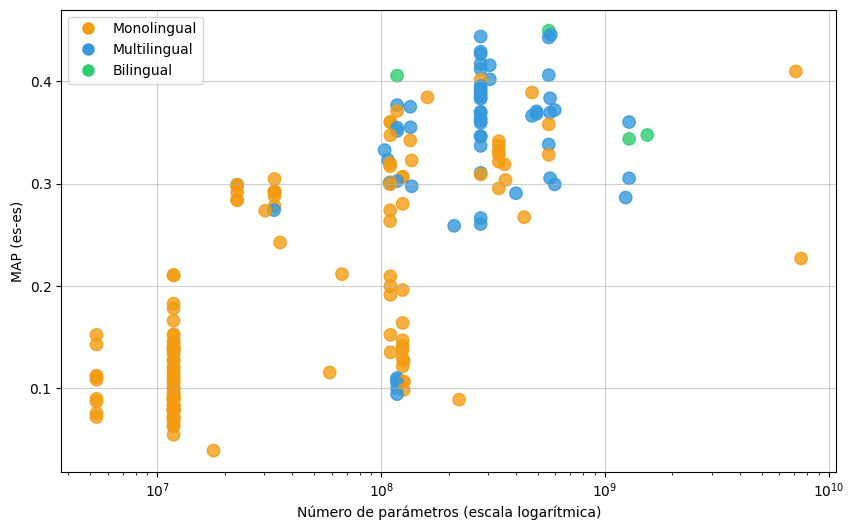
\includegraphics[width=0.9\textwidth]{imagenes/zero-shot-evaluation-plot.png}
    \caption{Resultados de los modelos preentrenados en evaluación Zero-Shot sobre la métrica \gls{MAP}. En el eje X se representan los modelos ordenados por su tamaño (número de parámetros) en escala logarítmica.}
    \label{fig:zero_shot_map}
\end{figure}

Podemos observar una clara predominancia de los modelos multilingües frente a los monolingües, a pesar que el conjunto de validación sobre el que han sido evaluados es integramente en español. Esto indica que los modelos multilingües han sido capaces de capturar representaciones efectivas para el idioma español, a pesar de no estar específicamente entrenados para él.

\section{Selección de modelos y entrenamiento}

Podemos observar en la tabla \ref{tab:top_10_zero_shot} los 10 mejores modelos obtenidos en la evaluación Zero-Shot\footnote{Podemos observar en la tabla \ref{tab:resultados_completos_modelos_zero_shot} el número de parámetros asociado a cada modelo, pudiendo constatar que se trata de modelos con arquitecturas y tamaños muy diversos.}. Cabe destacar que ninguno de ellos es monolingüe, sino que todos son modelos multilingües o bilingües que incluyen el español entre los idiomas con los que han sido entrenados, alineado con los resultados observados en la figura \ref{fig:zero_shot_map}.

\begin{table}[H]
    \centering
    \begin{tabular}{|l|l|l|}
        \hline
        \textbf{Modelo}                                             & \textbf{MAP} \\ \hline
        Lajavaness/bilingual-embedding-large                        & 0.4493       \\ \hline
        jinaai/jina-embeddings-v3                                   & 0.4453       \\ \hline
        chienpham/sts-multilingual-mpnet-base-v2                    & 0.4436       \\ \hline
        intfloat/multilingual-e5-large-instruct                     & 0.4426       \\ \hline
        AIDA-UPM/mstsb-paraphrase-multilingual-mpnet-base-v2        & 0.4287       \\ \hline
        shtilev/medical\_embedded\_v4                               & 0.4265       \\ \hline
        sentence-transformers/paraphrase-multilingual-mpnet-base-v2 & 0.4169       \\ \hline
        Alibaba-NLP/gte-multilingual-base                           & 0.4155       \\ \hline
        shtilev/medical\_embedded\_v5                               & 0.4117       \\ \hline
    \end{tabular}
    \caption{Top 10 modelos preentrenados en evaluación Zero-Shot ordenados por su métrica MAP.}
    \label{tab:top_10_zero_shot}
\end{table}

Para mayor legibilidad, de aquí en adelante nos referiremos a los modelos por su nombre, omitiendo el prefijo del autor/plataforma. Así, por ejemplo, el modelo \textit{Lajavaness/bilingual-embedding-large} será referido simplemente como \textit{bilingual-embedding-large}.

Se han considerado estos 10 modelos para su posterior ajuste fino mediante entrenamiento supervisado, utilizando el conjunto de datos de entrenamiento descrito en la sección \ref{sec:Conjuntos_de_datos}\todo{buscar o establecer definición de las fuentes de datos, ejemplos...}. Los modelos han sido entrenados durante una única época para evitar el sobreajuste, utilizando una tasa de aprendizaje de 5e-6 y un tamaño de batch de 16 muestras. Se ha utilizado la función de pérdida \gls{MNRL} descrita en la sección \ref{sec:Funciones_de_perdida}.


En la figura \ref{fig:finetuned_loss} se pueden observar las curvas de pérdida durante el entrenamiento de algunos de los modelos, descartando el entrenamiento en épocas adicionales debido al sobreajuste observado.

\begin{figure}[H]
    \centering
    \begin{minipage}{0.45\textwidth}
        \centering
        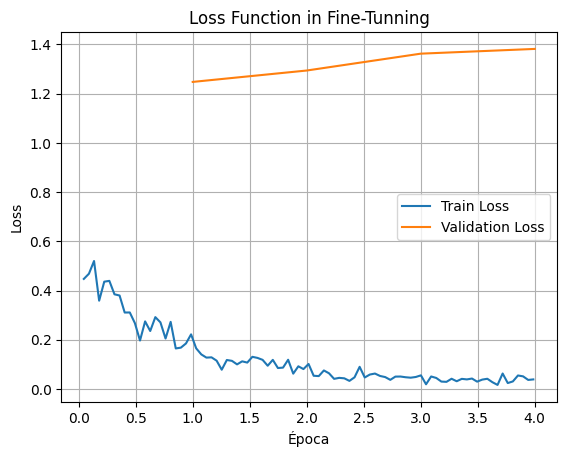
\includegraphics[width=\textwidth]{imagenes/training/shtilev-medical_embedded_v4.png}
    \end{minipage}
    \hfill
    \begin{minipage}{0.45\textwidth}
        \centering
        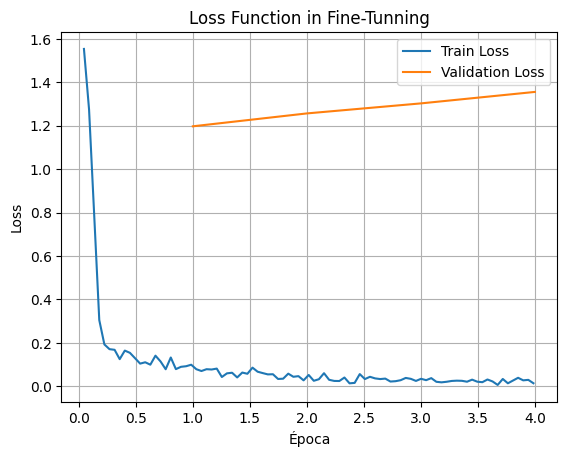
\includegraphics[width=\textwidth]{imagenes/training/intfloat-multilingual-e5-large-instruct.png}
    \end{minipage}
    \caption{Curvas de pérdida durante el entrenamiento de los modelos \textit{medical\_embedded\_v4} (izquierda) y \textit{multilingual-e5-large-instruct} (derecha) desde el comienzo del entrenamiento hasta la cuarta época. Se puede observar claramente el crecimiento en la pérdida de validación a partir de la primera época, indicando sobreajuste.}
    \label{fig:finetuned_loss}
\end{figure}

Los resultados obtenidos tras el entrenamiento de los modelos se pueden observar en la tabla \ref{tab:finetuned_results}. Se puede observar que los dos peores modelos, \textit{jina-embeddings-v3} y \textit{Linq-Embed-Mistral}, no han mejorado sus resultados, lo cual es debido a que no recibieron entrenamiento. Esto ha sucedido así debido a la configuración de ambos modelos, estando optimizados y cerrados para su uso en inferencia, lo que impide su ajuste mediante entrenamiento supervisado.

\begin{table}[H]
    \centering
    \begin{tabular}{rlrr}
        \hline
           & model\_name                                 & previous\_map & finetuned\_map \\
        \hline
        1  & bilingual-embedding-large                   & 0.4493        & 0.4902         \\
        2  & multilingual-e5-large-instruct              & 0.4426        & 0.4902         \\
        3  & gte-multilingual-base                       & 0.4155        & 0.4693         \\
        4  & paraphrase-multilingual-mpnet-base-v2       & 0.4169        & 0.4602         \\
        5  & mstsb-paraphrase-multilingual-mpnet-base-v2 & 0.4287        & 0.4589         \\
        6  & medical\_embedded\_v4                       & 0.4265        & 0.4580         \\
        7  & medical\_embedded\_v5                       & 0.4117        & 0.4568         \\
        8  & sts-multilingual-mpnet-base-v2              & 0.4436        & 0.4516         \\
        9  & jina-embeddings-v3                          & 0.4453        & 0.4453         \\
        10 & Linq-Embed-Mistral                          & 0.4095        & 0.4095         \\
        \hline
    \end{tabular}
    \caption{Resultados obtenidos tras el ajuste fino de los 10 mejores modelos preentrenados en evaluación Zero-Shot. Se muestran los valores de la métrica MAP antes y después del entrenamiento supervisado.}
    \label{tab:finetuned_results}
\end{table}

Se puede observar que la media de mejora tras el ajuste fino de los modelos ha sido de 3 puntos porcentuales en la métrica \gls{MAP}, lo que representa una mejora significativa en el desempeño de los modelos para la tarea que nos concierne.


\section{Ranking Fusion}

Una vez obtenidos los resultados de los modelos ajustados, se ha procedido a realizar una fusión de los rankings generados por los tres mejores modelos, que son \textit{bilingual-embedding-large}, \textit{multilingual-e5-large-instruct} y \textit{gte-multilingual-base}. La fusión de rankings se ha llevado a cabo mediante un análisis exhaustivo de técnicas y optimización de parámetros.

\subsection{Análisis de técnicas de fusión}

\subsubsection{Reciprocal Rank Fusion (RRF)}

Se ha utilizado la técnica de \gls{RRF} descrita en la sección \ref{sec:Rank_Fusion}, que ha demostrado ser efectiva en la combinación de múltiples rankings para mejorar la precisión de los resultados. Tras un análisis exhaustivo, se ha determinado que el valor óptimo para el parámetro $k$ es 5, lo que ha permitido maximizar la métrica \gls{MAP} obtenida tras la fusión. Se puede observar en la figura \ref{fig:rrf_k_analysis} el análisis realizado para la selección del valor óptimo de $k$.

\begin{figure}[H]
    \centering
    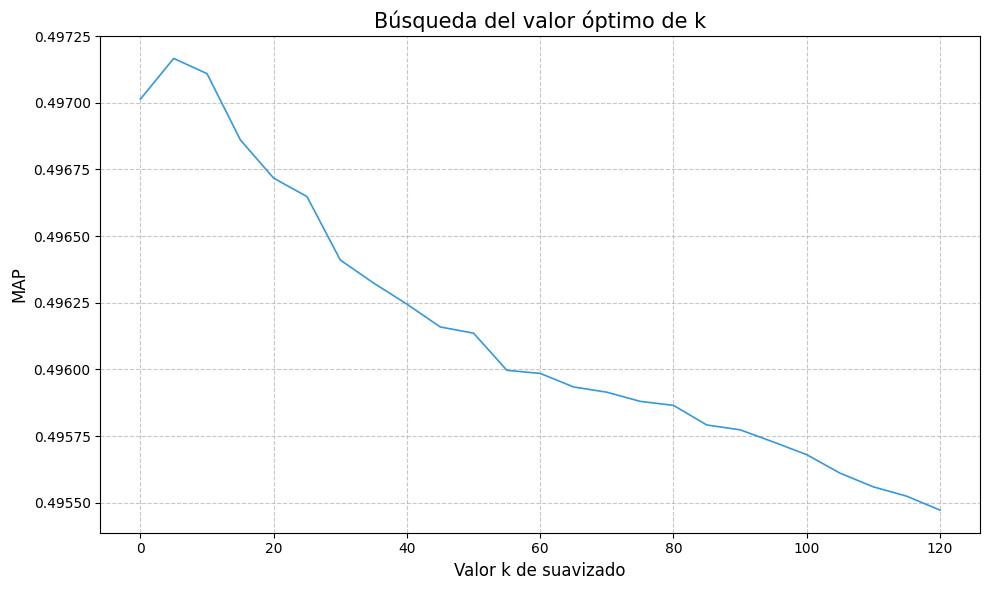
\includegraphics[width=0.7\textwidth]{imagenes/curva_optimizacion_k_fusion.png}
    \caption{Análisis del parámetro $k$ en la técnica de \gls{RRF} para la fusión de rankings. Se observa que el valor óptimo es 5, que maximiza la métrica \gls{MAP}.}
    \label{fig:rrf_k_analysis}
\end{figure}

Esta técnica ha supuesto una mejora en los resultados obtenidos, alcanzando un valor de \gls{MAP} de 0.49717, superando a los mejores modelos individuales tras el ajuste fino. 

\subsubsection{Mean Normalized Z-score}
%0.49896
Se ha explorado también la técnica de \gls{MNZ} para la fusión de rankings, que normaliza las puntuaciones de los documentos antes de combinarlas. Tras una normalización min-max, se ha aplicado la fórmula del \gls{MNZ} para combinar los rankings de los tres mejores modelos. Esta técnica ha permitido alcanzar un valor de \gls{MAP} de 0.49896, ligeramente superior al obtenido con \gls{RRF}.

\subsubsection{Weighted Sum}

Por último, se ha evaluado la técnica de \gls{WSum}, que asigna pesos específicos a cada modelo en función de su desempeño individual. Tras un análisis exhaustivo, se han asignado los siguientes pesos: 0.35 a \textit{bilingual-embedding-large}, 0.38 a \textit{multilingual-e5-large-instruct} y 0.27 a \textit{gte-multilingual-base}.

Esta técnica ha permitido alcanzar un valor de \gls{MAP} de 0.49953, siendo la mejor técnica de fusión evaluada.

\subsection{Arquitectura seleccionada}

Tras evaluar las tres técnicas de fusión de rankings, se ha seleccionado la técnica de \gls{WSum} como la más efectiva para nuestro caso de estudio, debido a que ha proporcionado el mejor desempeño en términos de la métrica \gls{MAP}. La asignación de pesos específicos a cada modelo ha permitido aprovechar sus fortalezas individuales, resultando en una mejora significativa en la precisión de los resultados obtenidos tras la fusión.


\section{Re-Ranking}